\documentclass{scrartcl}

\usepackage{ucs}
\usepackage[utf8x]{inputenc}
\usepackage[english]{babel}
\usepackage{graphicx}
\usepackage{amsmath}
\usepackage{amssymb}
\usepackage[ruled,linesnumbered]{algorithm2e}
\usepackage{hyperref}

\setlength\parindent{0pt}

\title{Effiziente Algorithmen \\ Zusammenfassung}
\author{Thomas Mohr}
\date{}

\begin{document}
\maketitle
\pagebreak
\tableofcontents
\pagebreak
\listofalgorithms
\pagebreak

\section{Grundlagen}

\subsection{Stable Matching}

\subsubsection{Praktisches Problem}

Ordne Medizinstudenten Praktikumsplätze in Krankenhäusern zu, wobei die gegenseitigen Präferenzen beachtet werden.

\subsubsection{Eingabe}

$ M = \{ m_1,\ldots,m_n \} $ (''Männer'') \\
$ W = \{ w_1,\ldots,w_n \} $ (''Frauen'') \\
jeder $ m \in M $ ordnet alle Elemente aus $ W $ nach Präferenz
jede $ w \in W $ ordnet alle Elemente aus $ M $ nach Präferenz

\subsubsection{Aufgabe}

Finde paarweise Zuordnung zwischen den Elementen aus $ M $ und $ W $, so dass für jeden $ m \in M $ und jede $ w \in W $, die nicht $ m $ zugeordnet ist, gilt (Stabilität):
\begin{enumerate}
	\item $ m $ zieht ihm zugeordnete $ w' $ gegenüber $ w $ vor, oder
	\item $ w $ zieht ihr zugeordneten $ m' $ gegenüber $ m $ vor
\end{enumerate}
Stabilität beschreibt hierbei, dass die Paarungen tatsächlich vorteilhaft sind für einen von beiden. D.h., wenn $ (m,w) $ ein Paar ist, aber $ m $ lieber ein Paar mit $ w' $ bilden würde, bzw. $ w $ lieber ein Paar mit $ m' $ bilden würde, so wäre ihre Verbindung instabil.

\subsubsection{Beispiel}

\begin{minipage}{.5\linewidth}
	\begin{align*}
		M = \{ X,Y,Z \} \\
		X: A < B < C \\
		Y: B < A < C \\
		Z: A < B < C
	\end{align*}
\end{minipage}
\begin{minipage}{.5\linewidth}
	\begin{align*}
		W = \{ A,B,C \} \\
		A: Y < X < Z \\
		B: X < Y < Z \\
		C: X < Y < Z
	\end{align*}
\end{minipage}

\begin{itemize}
	\item Zuordnung $ (X,C),(Y,B),(Z,A) $ \\
	Ist diese Zuordnung stabil? Nein! $ X $ zieht $ A $ vor und $ A $ zieht $ X $ vor.
	\item Zuordnung $ (X,A),(Y,B),(Z,C) $ \\
	Ist die Zuordnung stabil? Ja!
	\begin{enumerate}
		\item Niemand will mit $ Z $ oder $ C $ tauschen
		\item $ X $ hat Traumfrau
		\item $ Y $ hat Traumfrau
	\end{enumerate}
\end{itemize}

\subsubsection{Propose-\&-Reject}

\begin{algorithm}[H]
	alle $ m \in M $ und alle $ w \in W $ ''frei'' \\
	\While{$ \exists m \in M : m $ ist frei und $ \exists w \in W $ der $ m $ noch keinen Antrag gemacht hat}{
		$ w \leftarrow $ erste noch ''unbeantragte'' Frau in $ m $'s Präferenzfolge \\
		\If{$ w $ ist frei}{
			$ (m,w) $ wird Paar \\
			$ m \leftarrow $ ''verlobt'' \\
			$ w \leftarrow $ ''verlobt''
		}
		\ElseIf{$ w $ zieht $ m $ ihrem aktuellen Verlobten $ m' $ vor}{
			$ (m,w) $ wird Paar \\
			$ m \leftarrow $ ''verlobt'' \\
			$ w \leftarrow $ ''verlobt'' \\
			$ m' \leftarrow $ ''frei''
		}
		\Else{$ w $ lehnt $ m $ ab}
	}
	\caption{Propose-\&-Reject}
\end{algorithm}

\begin{itemize}
	\item Propose--Reject findet immer ein \textbf{perfektes Matching}, das stabil ist, und benötigt dazu $ \leq n^2 $ \textbf{Durchläufe} der while-Schleife.
	\item Jeder Mann bekommt die bestmögliche Frau zugeordnet (''männeroptimal'').
	\item Jede Frau bekommt den schlechtestmöglichen Mann zugeordnet.
\end{itemize}

\subsubsection{5 respräsentative Probleme}
\begin{enumerate}
	\item Interval Scheduling
	\begin{itemize}
		\item Eingabe: Intervalle mit Start- \& Endzeiten
		\item Aufgabe: Finde größtmögliche Menge nichtüberlappender Intervalle
		\item Beispiel für Greedy \\
		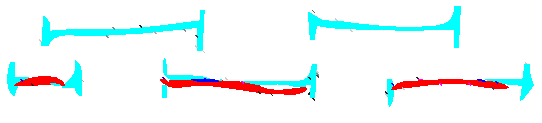
\includegraphics[width=\linewidth]{figures/interval-scheduling.pdf}
	\end{itemize}
	\item Gewichtetes Interval Scheduling
	\begin{itemize}
		\item Eingabe: Intervalle mit Start- \& Endzeiten und positiven Gewichten
		\item Aufgabe: Finde Lösung mit größtmöglichem Gesamtgewicht
		\item Beispiel für dynamisches Programmieren: \\
		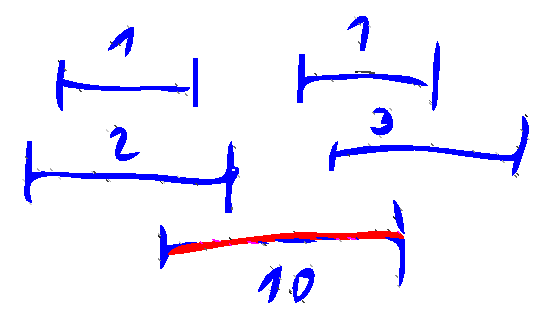
\includegraphics[width=\linewidth]{figures/gewichtetes-interval-scheduling.pdf}
	\end{itemize}
	\item Bipartites Matching
	\begin{itemize}
		\item Eingabe: Bipartiter Graph
		\item Aufgabe: Finde größtmögliche ''unabhängige'' (keine gemeinsamen Endpunkte) Kantenmenge
		\item Beispiel für Netzwerkflüsse: \\
		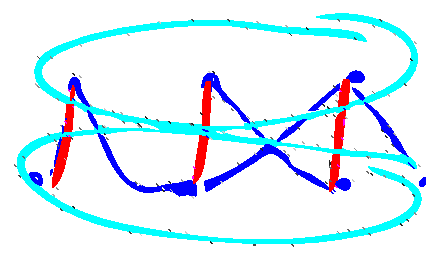
\includegraphics{figures/bipartites-matching.pdf}
	\end{itemize}
	\item Independent set
	\begin{itemize}
		\item Eingabe: Ungerichteter Graph
		\item Aufgabe: Finde größtmögliche ''unabhängige'' (paarweise nicht benachbarte) Knotenmenge
		\item Beispiel (NP-schwer): \\
		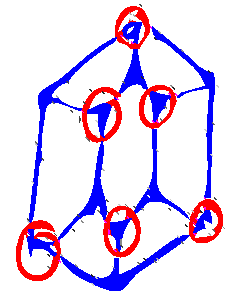
\includegraphics{figures/independent-set.pdf}
		\item Vorige Probleme sind Spezialfälle von \textbf{Independent Set}
	\end{itemize}
	\item Competitive Facility Location
	\begin{itemize}
		\item Eingabe: Knotengewichteter Graph
		\item Regeln: Zwei Spieler wählen alternierend Knoten; gewählter Knoten wird samt Nachbarn gelöscht.
		\item Ziel: Spieler 1 will Knoten so wählen, dass Spieler 2 möglichst wenige Pnkte macht
		\item Beispiel (PSPACE-vollständig): \\
		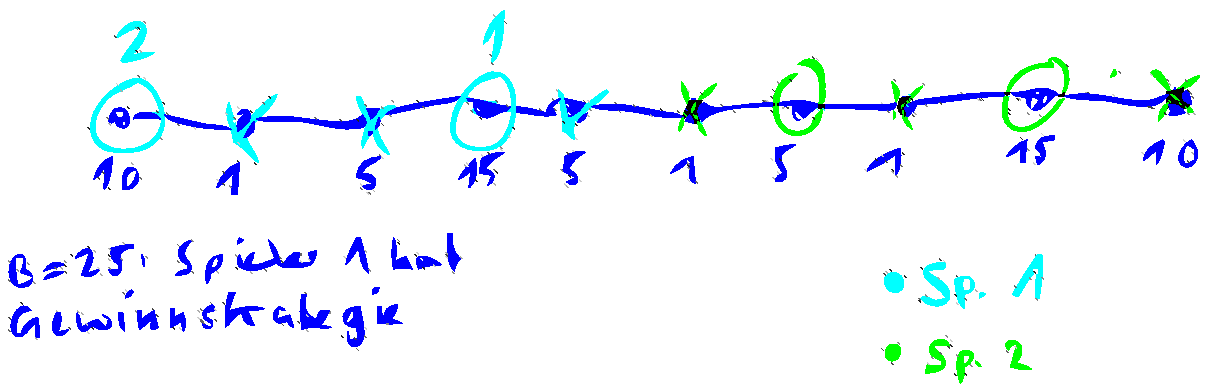
\includegraphics[width=\linewidth]{figures/competitive-facility-location.pdf}
	\end{itemize}
\end{enumerate}

\subsection{Zentrale Konzepte \& Konventionen}

\begin{itemize}
	\item Ziel \textbf{effizienter} Algorithmen: \textbf{polynomielle Laufzeit}, d.h. es existieren Konstanten $ c,d $, so dass der Algorithmus bei Eingabegröße $ n $ nach $ c \cdot n^d $ Schritten terminiert.
	\item Man beachte: \textbf{Worst-Case Analyse}
\end{itemize}

\subsubsection{$ \mathcal{O} $-Notation}

\begin{itemize}
	\item $ T(n) = \mathcal{O}(f(n)) $ falls $ \exists c > 0, n_0 \geq 0: \forall n \geq n_0 : T(n) \leq c \cdot f(n) $ \\
	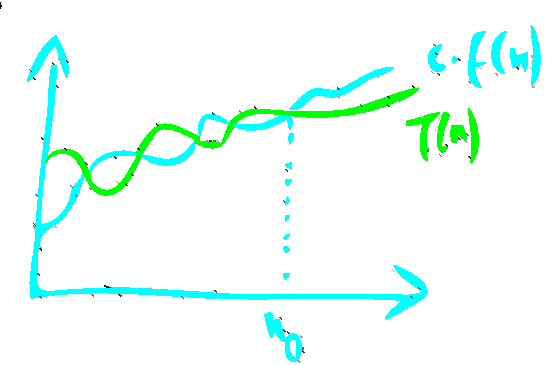
\includegraphics[width=\linewidth]{figures/o-notation.pdf}
	\item $ T(n) = \Omega(f(n)) $ falls $ \exists c > 0, n_0 \geq 0 : \forall n \geq n_0: T(n) \geq c \cdot f(n) $
	\item $ T(n) = \Theta(f(n)) $ falls $ T(n) = \mathcal{O}(f(n)) $ und $ T(n) = \Omega(f(n)) $ \\
	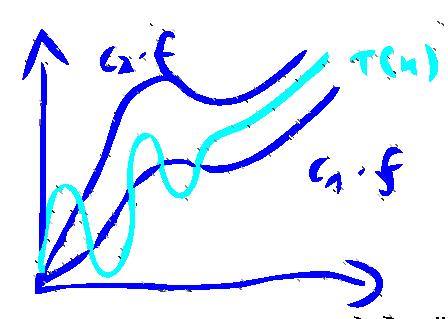
\includegraphics[width=\linewidth]{figures/theta.pdf}
	\item $ T(n) = o(f(n)) $ falls $ \forall c > 0 : \exists n_0 \geq 0 \forall n \geq n_0 : T(n) < c \cdot f(n) $
	\item $ T(n) = \omega(f(n)) $ falls $ f(n) = o(T(n)) $
\end{itemize}

Wenn die Eingabe $ n $ groß genug wird wächst $ T $
\begin{itemize}
	\item $ T(n) = \mathcal{O}(f(n)) $ \hfill nicht schneller
	\item $ T(n) = \Omega(f(n)) $ \hfill nicht langsamer
	\item $ T(n) = \Theta(f(n)) $ \hfill genauso schnell
	\item $ T(n) = o(f(n)) $ \hfill echt langsamer
	\item $ T(n) = \omega(f(n)) $ \hfill echt schneller
\end{itemize}
als $ f $.

\subsection{Graphen}

\begin{itemize}
	\item $ G = (V,E) $
	\item Konvention: $ n .= \mid V \mid, m:= \mid E \mid $
	\item Gerichteter Graph: $ e \in E $ mit $ e = (u,v), u, v \in V $ (geordnetes Paar) \\
	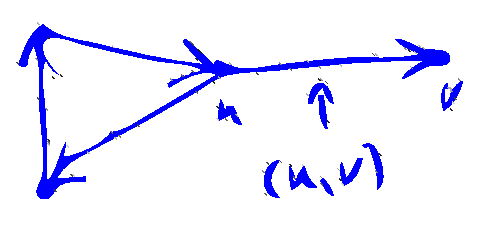
\includegraphics[width=\linewidth]{figures/gerichteter-graph.pdf}
	\item Ungerichteter Graph: $ e \in E $ mit $ e = \{ u,v \}, u, v \in V $ (ungeordnetes Paar) \\
	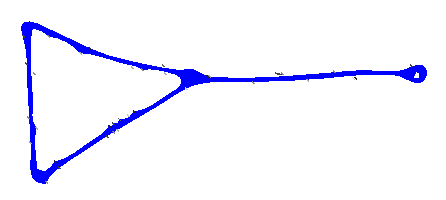
\includegraphics[width=\linewidth]{figures/ungerichteter-graph.pdf}
\end{itemize}

\subsubsection{Repräsentation}

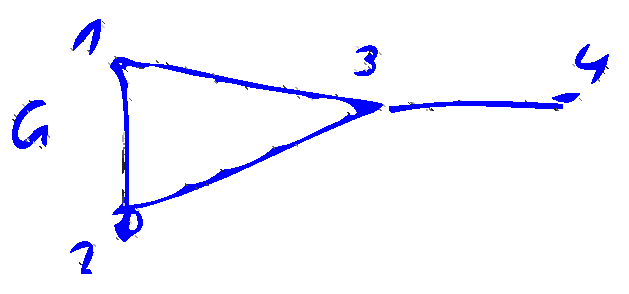
\includegraphics[width=\textwidth]{figures/graph.pdf}

\begin{itemize}
	\item Adjazenzmatrix
	\begin{itemize}
		\item $ n \times n $ 0/1-Matrix
		\item $ A_{i,j} = 1 \iff \{ v_i,v_j \} \in E $
		\item Hoher Speicherbedarf für Graphen mit wenigen Kanten (''dünn'', ''sparse'')
	\end{itemize}
	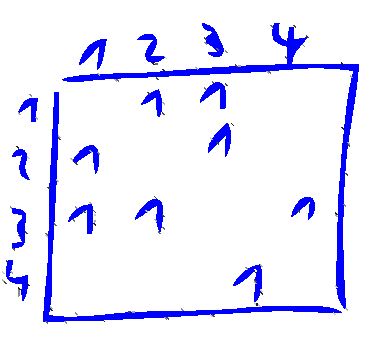
\includegraphics{figures/adjazenz-matrix.pdf}
	\item Adjazenzliste
	\begin{itemize}
		\item Array/Liste von Nachbarn für jeden Knoten
		\item Jeder Array-Eintrag führt zur Liste von Nachbarn
	\end{itemize}
	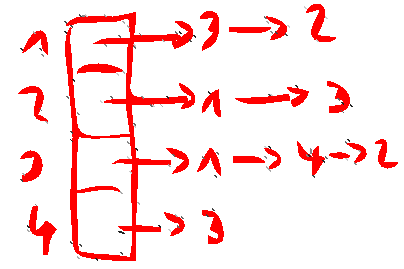
\includegraphics{figures/adjazenz-liste.pdf}
\end{itemize}

\subsubsection{Bekannte Begriffe}

\begin{itemize}
	\item Pfad: Folge von Knoten, aufeinanderfolgende sind benachbart \\
	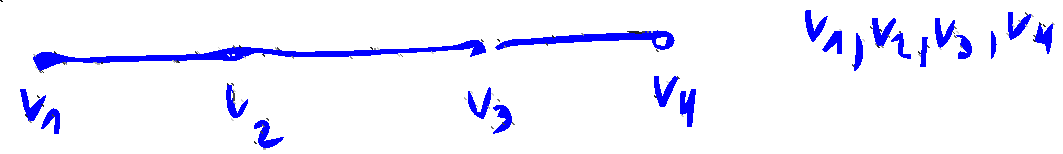
\includegraphics[width=\linewidth]{figures/pfad.pdf}
	\item Kreis: Pfad $ v_1,\ldots,v_l $ mit $ v_1=v_l $ \\
	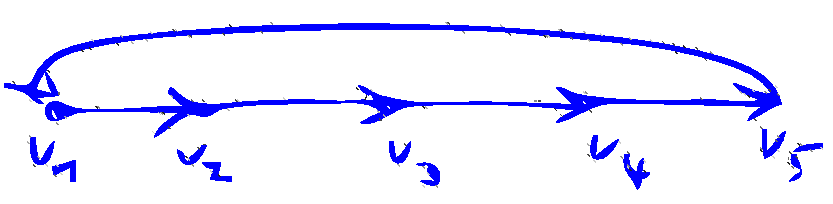
\includegraphics[width=\linewidth]{figures/kreis.pdf}
	\item Ungerichteter zusammenhängender Graph: Zwischen allen Knotenpaaren existiert ein Pfad \\
	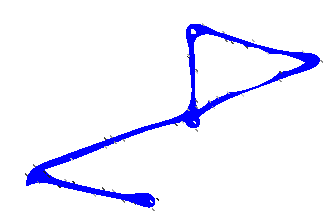
\includegraphics{figures/ungerichteter-zusammenhaengender-graph.pdf}
	\item Baum: Ungerichtet, kreisfrei, zusammenhängend \\
	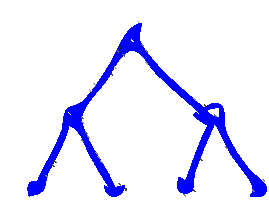
\includegraphics{figures/baum.pdf}
\end{itemize}

\subsubsection{Graphtraversierung}

\paragraph{Breitensuche (BFS)}

\begin{itemize}
	\item Idee
	\begin{itemize}
		\item Beginne am Startknoten $ s $
		\item Durchforste Graph ''schichtweise'' (erst Abstand 1 zu $ s $, dann Abstand 2, usw.)
	\end{itemize}
	\item Wichtige Datenstruktur: Schlange (FIFO)
	\item BFS kann in $ \mathcal{O}(n+m) $ Zeit durchgeführt werden
	\item Eventuell hoher Speicherbedarf
	\item Mit BFS findet man alle kürzesten Pfade ausgehend von $ s $
\end{itemize}

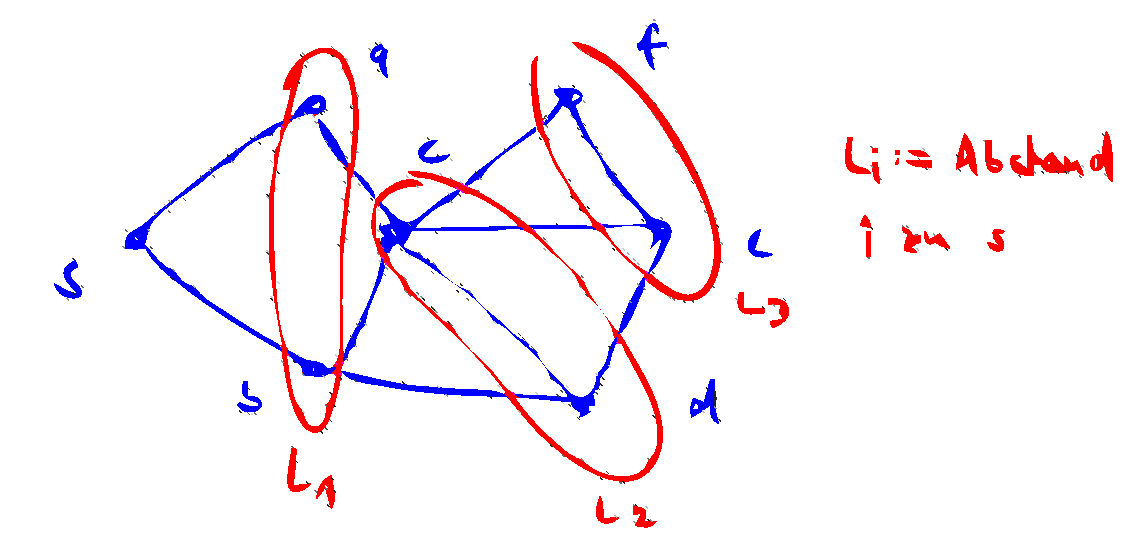
\includegraphics[width=\linewidth]{figures/bfs.pdf}

\paragraph{Tiefensuche (DFS)}\mbox{} \\
\begin{algorithm}[H]
	\KwIn{Startknoten $ u $}
	$ R \leftarrow \emptyset $ \\
	Markiere $ u $ als besucht \\
	$ R \leftarrow R \cup \{ u \} $ \\
	\ForEach{$ \{ u,v \} \in E $}{
		\If{$ v $ nicht besucht}{
			\texttt{DFS}($ v $)
		}
	}
	\KwRet{$ R $}
	\caption{DFS}
\end{algorithm}

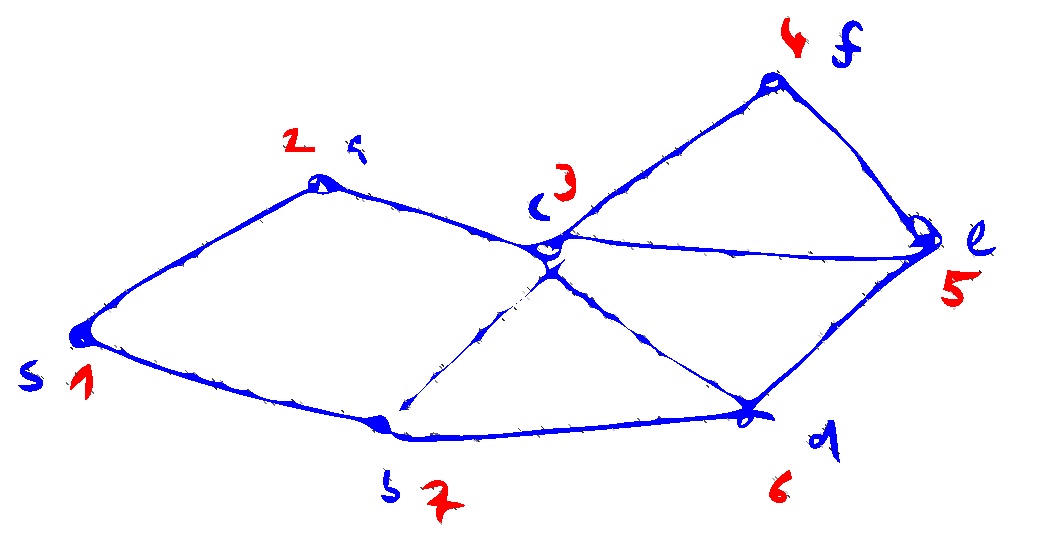
\includegraphics[width=\linewidth]{figures/dfs.pdf}

\begin{itemize}
	\item DFS kann in $ \mathcal{O}(n+m) $ Zeit durchgeführt werden.
	\item DFS findet in der Regel keine kürzesten Wege.
	\item Anwendung z.B. beim Finden von Zusammenhangskomponenten.
\end{itemize}

\subsection{Bipartite Graphen}

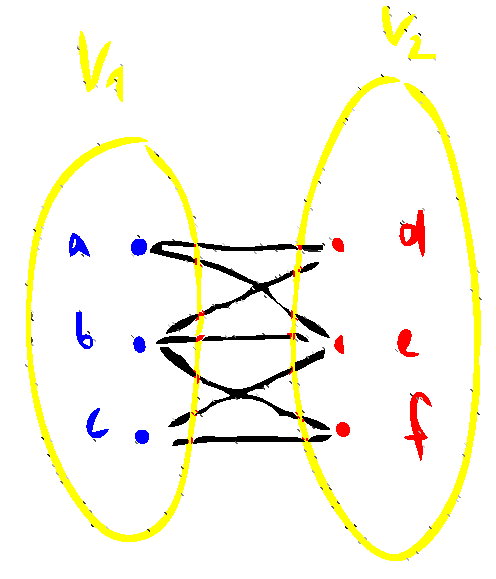
\includegraphics{figures/bipartiter-graph.pdf}

\begin{itemize}
	\item Ein Graph $ G = (V,E) $ ist \textbf{bipartit}, falls $ V = V_1 \cup V_2 $ mit $ V_1 \cap V_2 = \emptyset $ und $ E \subseteq V_1 \times V_2 $.
	\item Äquivalent:
	\begin{itemize}
		\item $ G $ ist zweifärbbar \\
		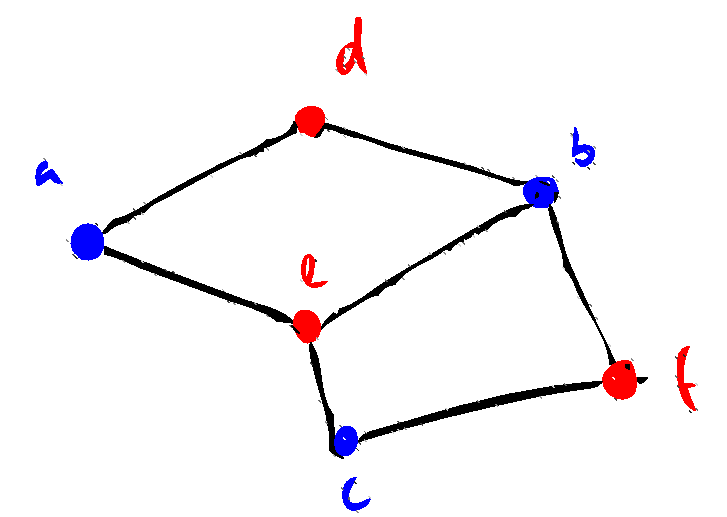
\includegraphics{figures/zweifaerbbar.pdf}
		\item $ G $ hat keinen Kreis ungerader Länge \\
		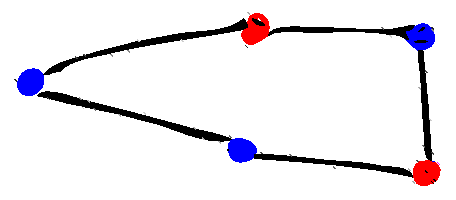
\includegraphics[width=\linewidth]{figures/kreis-ungerader-laenge.pdf}
	\end{itemize}
\end{itemize}

\subsubsection{Starker Zusammenhang}

\begin{itemize}
	\item Ein gerichteter Graph heißt \textbf{stark zusammenhängend}, falls jedes Knotenpaar \textbf{wechselseitig} durch jeweils mind. einen gerichtetetn Pfad verbunden ist.
	\item Es kann in $ \mathcal{O}(n+m) $ Zeit festgestellt werden, ob ein Graph $ G = (V,E) $ stark zusammenhängend ist.
	\item Beispiel
	\begin{itemize}
		\item Stark zusammenhängend \\
		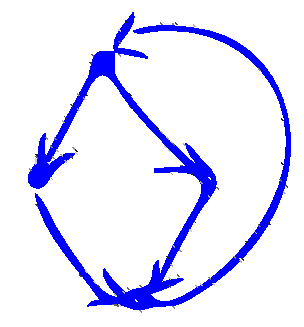
\includegraphics{figures/stark-zusammenhaengend.pdf}
		\item Nicht stark zusammenhängend \\
		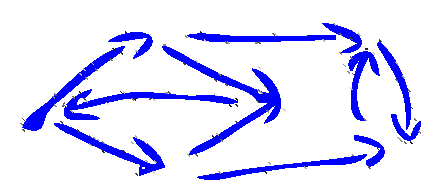
\includegraphics[width=\linewidth]{figures/nicht-stark-zusammenhaengend.pdf}
	\end{itemize}
\end{itemize}

\subsubsection{DAG's \& topologische Sortierungen}

\begin{itemize}
	\item Sei $ G = (V,E) $ ein gerichteter Graph. Eine \textbf{topologische Sortierung} ist eine totale Ordnung $ v_1,v_2,\ldots,v_n $ mit Knoten aus $ V $, so dass für jede Kante $ (v_i,v_j) \in E $ gilt: $ i < j $.
	\item DAG: ''directed acyclic graph'': gerichteter, azyklische Graph
	\item Beispiel: \\
	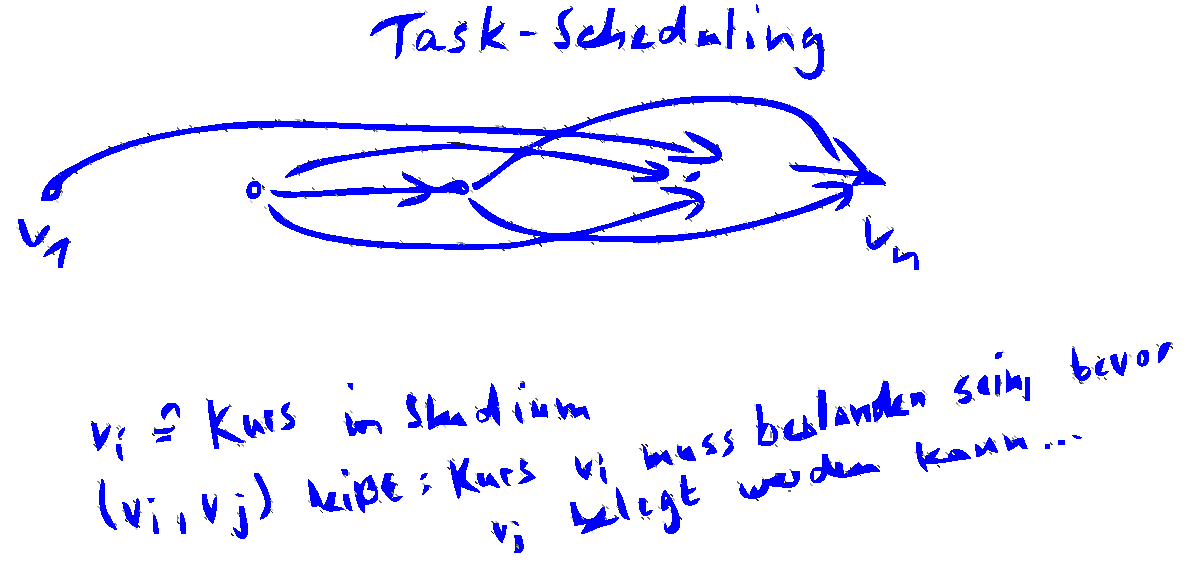
\includegraphics[width=\linewidth]{figures/task-scheduling.pdf}
	\item $ G $ ist gerichtet azyklisch $ \iff G $ hat top. Sortierung
	\item Eine topologische Sortierung eines Graphen $ G $, falls existierend, kann in $ \mathcal{O}(n+m) $ Zeit gefunden werden. Beweisidee:
	\begin{enumerate}
		\item Finde $ v \in V $ ohne Eingangskante
		\item Setze $ v $ an Spitze der Sortierung
		\item Lösche $ v $
		\item Finde Sortierung von ''$ G - v $'' rekursiv und setze diese hinter $ v $
	\end{enumerate}
\end{itemize}

\end{document}